\PassOptionsToPackage{hyphens}{url}
\documentclass[review,authoryear]{elsarticle}

\usepackage{amsmath,amssymb,amsfonts,amsthm}
\usepackage{booktabs}
\usepackage{tikz}
\usepackage{hyperref}
\hypersetup{hidelinks}

\usetikzlibrary{positioning,calc}

\makeatletter
\def\input@path{{paper/}{}}
\makeatother

\newtheorem{assumption}{Assumption}
\let\lemma\undefined
\let\endlemma\undefined
\newtheorem{lemma}{Lemma}
\newtheorem{proposition}{Proposition}
\newtheorem{theorem}{Theorem}
\newtheorem{corollary}{Corollary}
\newtheorem{remark}{Remark}
\theoremstyle{definition}
\newtheorem{definition}{Definition}
\theoremstyle{plain}
\newcommand{\Description}[1]{}

\begin{document}

\begin{frontmatter}

\title{Profitable Cheap Talk and Zero-Retaliation Rent: Why Trust-Restoring Signals Fail Before Common Knowledge}

\author{Anonymous Author(s)}
\address{Submission \#XXX, USA}

\begin{abstract}
We study a signaling environment in which the messages by which posteriors would become common knowledge are themselves profitable to distort. A sender classifies a payoff-relevant object that is not a strategic player and therefore cannot impose refusal, exit, sanction, litigation, or retaliation costs on false classification. Anthropomorphic AI marketing is the leading application. At this zero-retaliation boundary, trust-restoring messages are not merely cheap talk; they are profitable cheap talk. We show that pooling survives neologism-proofness: every trust-restoring message available to the high-governance type is profitably shadowable by the low-governance type. Voluntary non-arbitrage is therefore not incentive compatible. Separation requires externally imposed signal costs satisfying single crossing, such as audit trails, sanctionable inconsistency, and auditable records. A dynamic extension embeds the baseline game in an endogenous trust-capital law of motion and shows that cheap anthropomorphic signals, user habituation, and delayed harms do not by themselves break pooling: when the semantic premium and engagement reinforcement offset bounded asynchronous shocks, the pooling interval is almost surely forward-invariant.
\end{abstract}

\begin{keyword}
Signaling games \sep profitable cheap talk \sep zero-retaliation rent \sep endogenous trust \sep dynamic pooling \sep neologism-proofness \sep costly signaling \sep auditable records
\end{keyword}

\end{frontmatter}

% !TEX root = ../arbitrage.tex
\section{Introduction: Before Common Knowledge}
\label{sec:introduction}

Aumann showed that rational agents with a common prior cannot agree to disagree once their posteriors are common knowledge \citep{aumann1976agreeing}. But how do posteriors become common knowledge when the messages that would reveal them are themselves profitable to distort? They often do not. In profitable cheap-talk environments, trust-restoring messages are rationally mimicked by the very types they are meant to exclude.

Anthropomorphic AI marketing is a limit case because the classified object is payoff-relevant but cannot retaliate. A firm can sell the system as a companion, tutor, or collaborative agent in the consumption channel while describing the same system as a mere tool in liability-facing channels. The resulting surplus is \emph{zero-retaliation rent}: a premium earned on a classification boundary that carries no signal cost from the classified object. Standard cheap talk assumes costless messages. This paper studies a more pathological case: messages whose production cost is zero but whose equilibrium payoff is positive. The signal is not merely free to send; it is profitable to send.

The failure studied here occurs before Aumann agreement can begin. The problem is not that rational agents continue to disagree after posteriors become common knowledge. It is that the messages that would make posteriors common knowledge are themselves rent-generating. When a low-governance sender can profit from sending the same trust-restoring message as a high-governance sender, and when the classified object cannot impose retaliation costs on that message, truthful restraint is not an equilibrium strategy. The result is profitable cheap talk.

The contribution is five concrete claims:
\begin{enumerate}
    \item profitable cheap talk at the zero-retaliation boundary: the anthropomorphic signal has negative net cost for both governance types because the classified object cannot retaliate;
    \item neologism-proof shadowing: every trust-restoring message available to the high-governance type is profitably shadowable, so voluntary non-arbitrage is not incentive compatible;
    \item cost-imposed common-knowledge formation: separation requires externally imposed signal costs satisfying single crossing;
    \item pricing the ontological spread: sanctionable inconsistency, audit requirements, and auditable records each close a different term of the low-type arbitrage spread, and their necessity and sufficiency conditions are stated as a unified pricing proposition;
    \item dynamic extension: endogenous trust dynamics can lock in pooling, history-dependent trust-restoring messages remain shadowable, and dynamic separation requires an externally priced single-crossing wedge.
\end{enumerate}

The paper organizes the mathematics into a baseline proposition and dynamic extensions of the same signaling problem. Proposition~\ref{prop:pooling-pbe} establishes pooling on profitable cheap talk as a Perfect Bayesian Equilibrium. Theorem~\ref{thm:zero-retaliation-shadowing} proves that the pooling equilibrium is neologism-proof at the zero-retaliation boundary due to profitable shadowing. Theorem~\ref{thm:audit-cost-separation} proves cost-imposed common-knowledge formation under single crossing. Section~\ref{sec:trust-dynamics} then embeds the same incentives in a trust-capital state equation and proves dynamic pooling invariance, dynamic shadowing, and externally priced dynamic separation: history and delayed harms do not cure pooling unless some signal cost, audit price, or sanctionable inconsistency changes the Bellman value wedge.
% !TEX root = ../arbitrage.tex
\section{Model: Payoff-Relevant Non-Player as the Negative-Cost Signal Environment}
\label{sec:three-sided}

\begin{table}[t]
\centering
\scriptsize
\setlength{\tabcolsep}{2pt}
\renewcommand{\arraystretch}{1.2}
\begin{tabular}{@{}c|c|c@{}}
 & \textbf{Comply} & \textbf{Resist} \\
\hline
\textbf{Objectify} &
$(L+Sec,-C_{sub})$ &
$(L+Sec-C_{enf},-C_{sub}-C_{res})$ \\
\hline
\textbf{Recognize} &
$(Eth-Sec,+V)$ &
$(Eth-Sec,+V)$ \\
\end{tabular}
\caption{The inadequate dyadic model. The static Nash matrix is retained only
as a foil: it omits private types, public messages, posterior beliefs, and the
regulatory channel through which ontological claims become governable.}
\label{tab:dyadic-nash}
\end{table}

The standard starting point for ontological conflict is a dyadic observer--subject model; Table~\ref{tab:dyadic-nash} compresses that foil into a simultaneous Nash matrix that identifies a real temptation but omits types, messages, beliefs, and the regulatory channel. The more basic problem is the player set. In anthropomorphic AI markets, the system is the object around which strategic claims are made, but it is not a strategic player: it has no channel through which to impose costs on those claims.  At the zero-retaliation limit, this cost class is absent. What the stylized governance setting therefore requires is a three-sided structure: a Firm ($F$) that produces ontological claims, a User ($U$) that consumes them, and a Regulator ($R$) whose posterior over firm type determines whether the claims become governable. This section fixes the player intuition that the formal apparatus of Section~\ref{sec:bayesian} then makes precise.

\subsection{The Firm Side}
\label{subsec:firm-side}

A firm deploying a model has private knowledge of two parameters: its internal \emph{governance type} $\theta_F$ (the degree of investment in evaluations, red-teaming, and post-deployment monitoring) and the system's \emph{opacity} $\theta_S$ (the extent to which capability claims can be checked from outside). Both are unobservable to users and to regulators. What is observable is the firm's \emph{message}: a pair of public artefacts---marketing copy and policy/liability documentation---which together constitute the firm's signal $m_F$.

The signal admits two stable poles. \emph{Anthropomorphic marketing} attributes agency, judgment, or care to the system in ways that warrant a relational reading. \emph{Deflationary policy} disclaims exactly those attributes in ways that warrant a tool reading. The firm enjoys an \emph{ontological premium}: a utility surplus that accrues when the system is priced as agent in the consumption channel (driving willingness-to-pay and engagement) while being priced as tool in the liability channel (limiting redress). The premium is rent earned on a category boundary the firm itself does not have to defend. This is not a claim about firm pathology; it is a claim about the payoffs any firm faces under the present signal-cost structure. A firm with $\theta_F = \mathsf{H}$ that elected deflationary marketing would forfeit revenue to a competitor who did not, absent an external instrument that taxes the asymmetry.

\subsection{The User Side}
\label{subsec:user-side}

Users carry a private \emph{vulnerability type} $\theta_U$ that aggregates affective need, isolation, and the marginal value of a high-availability interlocutor. Their action $m_U \in \{\text{invest}, \text{detach}\}$ is the decision to extend or withhold investment: to act on the anthropomorphic signal or to discount it. The signal is observable, but the type is not. Users cannot inspect training data, evaluations, or internal incident reports; their evidence is the firm's message and the system's behaviour, both of which are jointly designed. This information asymmetry compounds because the harms of mis-investment are \emph{asynchronous}: the cost of acting on the anthropomorphic signal falls due in episodes (model deprecations, persona changes, refusals at moments of acute need) that may be separated from the original investment by months. A risk-neutral user under cheap-talk signals will rationally invest, because the immediate utility of invest exceeds the discounted expected cost of liquidation. Section~\ref{subsec:sanctionable-inconsistency} illustrates the consumer-side informational asymmetry with a concrete marketing--documentation example.

\subsection{The Regulator Side and the Public Channel}
\label{subsec:regulator-side}

A regulator $R$ chooses among \emph{inspect}, \emph{sanction}, and \emph{abstain}, conditional on a posterior over $\theta_F$ and $\theta_S$ formed from the firm's public messages and from an exogenous public signal $z$. The regulator's private type $\theta_R$ is \emph{bandwidth}: the capacity, technical and institutional, to discriminate genuine capability claims from cheap-talk ones. A high-bandwidth regulator can read whitepapers, commission audits, and detect inconsistency across the firm's two channels; a low-bandwidth regulator must rely on the channel $z$.

The public channel $z$ is the aggregate output of journalism, academic critique, civil-society advocacy, and incident reporting. We treat it as a noisy estimator of $\theta_F$: it shifts $R$'s posterior but does not deliver verdicts. Folding publics into $R$ this way is deliberate. Publics rarely have standing to sanction; they have standing to be \emph{heard}, and the channel through which they are heard is the regulator's information environment. Treating intellectuals and affected communities as autonomous players would over-parameterise the model without changing its qualitative behaviour: in every equilibrium we examine, what publics do is move $R$'s posterior; what changes the firm's behaviour is what $R$ does next.

The three-sided structure thus admits a single arbitrage logic. The firm earns rent on the spread between two ontological claims it makes about the same artefact. The user supplies the demand that makes the spread profitable. The regulator, in the absence of a verification mechanism that ties the two claims together, lacks an off-path belief stringent enough to deter the spread. The remainder of the paper formalises this structure (Section~\ref{sec:bayesian}), shows why trust-restoring messages fail (Section~\ref{sec:shadowing}), explains why profitable cheap talk persists (Section~\ref{sec:persistence}), and shows how its signal-cost structure may be redesigned (Section~\ref{sec:mechanism}).

\paragraph{Informal preview of the equilibrium analysis.}
A firm's governance quality is its private information. Under current conditions, describing an AI system as a companion or agent has zero production cost and positive continuation value. Because the signal is rent-generating for both governance types, it carries no type information: users cannot distinguish careful firms from careless ones, and regulators cannot justify the cost of inspection. This is the pooling equilibrium. Separation requires pricing the signal. If anthropomorphic marketing is valid only when paired with an audit trail---evaluation records, capability logs, incident reports---and if the cost of producing that trail is lower for firms that actually invested in governance (the single-crossing condition), then a threshold audit intensity exists above which low-governance firms will not imitate and below which high-governance firms can still afford to signal. A further asymmetry governs the size of the arbitrage premium itself. In prior recognition games, the classified subject retained a non-zero capacity to impose costs on the arbitrageur, which discounted the premium. The AI case is the limit where the subject's retaliation capacity is zero: the system has no independent channel through which to impose costs on the firm, leaving the ontological premium unconstrained. This structural boundary is formalized in Section~\ref{sec:bayesian}.
% !TEX root = ../arbitrage.tex
\section{Baseline Pooling: Rational Arbitrage, Not Moral Failure}
\label{sec:bayesian}

This section formalizes the three-sided market dynamics as a sequential signaling game under incomplete information. 

\subsection{Model}

\textbf{Players.} The strategic players are a Firm ($F$), a User ($U$), and a Regulator ($R$). The AI system is not a player but an object of classification. Publics enter as a noisy exogenous signal $z \in Z$. 

\textbf{Type Spaces.} Nature draws private types from a common prior $\pi$ over $\Theta = \Theta_F \times \Theta_U \times \Theta_R \times \Theta_S$. The firm's governance type is $\theta_F \in \{\mathsf{H},\mathsf{L}\}$. The user's vulnerability type is $\theta_U \in \{\mathsf{V},\mathsf{N}\}$. The regulator's bandwidth type is $\theta_R \in \{\mathsf{B},\bar{\mathsf{B}}\}$. The system-opacity parameter $\theta_S$ is private to $F$.

\textbf{Baseline Message Spaces.} In the unpriced baseline, the firm chooses $m_F \in \{a,p\}$, where $a$ is anthropomorphic marketing and $p$ is policy-deflationary positioning. The audit-augmented message space is introduced only in Theorem~\ref{thm:audit-cost-separation}, because audit intensity is an externally imposed signal cost rather than part of the cheap-talk baseline. The user chooses $m_U \in \{i,d\}$ (invest or detach). The regulator chooses $m_R \in \{x,s,o\}$ (inspect, sanction, or abstain).

\textbf{Timing.} 
1. $F$ observes $(\theta_F,\theta_S)$ and sends $m_F$.
2. $U$ observes $m_F$ and $\theta_U$, then sends $m_U$.
3. $R$ observes $(m_F,m_U,z)$ and $\theta_R$, then chooses $m_R$.

\textbf{Histories.} The user's public history is $h_U = (m_F)$, and the regulator's is $h_R = (m_F, m_U, z)$.

\textbf{Strategies.} A firm strategy $\sigma_F: \Theta_F \times \Theta_S \to \Delta(\{a,p\})$. A user strategy $\sigma_U: \{a,p\} \times \Theta_U \to \Delta(\{i,d\})$. A regulator strategy $\sigma_R: \{a,p\} \times \{i,d\} \times Z \times \Theta_R \to \Delta(\{x,s,o\})$.

\textbf{Beliefs.} The user forms posterior $\mu_U(\theta_F, \theta_S \mid h_U)$. The regulator forms posterior $\mu_R(\theta_F, \theta_S \mid h_R)$.

\textbf{Payoff Functions.} 
We consolidate the payoffs for Firm, User, and Regulator into the following block:
\begin{align*}
u_F(m_F, m_U, m_R) &= 
\begin{cases}
\Delta_F^S - c_{\theta_F}(m_F) - P(m_R) & \text{if } m_F=a, m_U=i \\
- c_{\theta_F}(m_F) - P(m_R) & \text{otherwise}
\end{cases} \\
u_U(m_F, m_U, \theta_F) &= 
\begin{cases}
B_{\theta_U} & \text{if } m_U=i, \theta_F=\mathsf{H} \\
B_{\theta_U} - H_{\theta_U} & \text{if } m_U=i, \theta_F=\mathsf{L} \\
0 & \text{if } m_U=d
\end{cases} \\
u_R(m_F, m_U, m_R, \theta_F) &=
\begin{cases}
-K_{\theta_R} + D_R & \text{if } m_R \in \{x,s\}, \theta_F=\mathsf{L} \\
-K_{\theta_R} & \text{if } m_R \in \{x,s\}, \theta_F=\mathsf{H} \\
0 & \text{if } m_R = o
\end{cases}
\end{align*}
where $\Delta_F^S$ is the ontological premium, $c_{\theta_F}(m_F)$ is the production or verification cost of the signal, $P(m_R)$ is the penalty if $R$ sanctions, $B_{\theta_U}$ is the immediate benefit of investment, $H_{\theta_U}$ is the future harm of false investment, $K_{\theta_R}$ is $R$'s inspection cost, and $D_R$ is $R$'s payoff from catching a low-governance firm.  The object that matters for the paper is the signal's \emph{net} cost:
\[
\operatorname{NetCost}_{\theta}(a)
:=
c_{\theta}(a)-\Delta_F^S .
\]
At the zero-retaliation boundary, we have $\Delta_F^S=\Delta_F$, so Assumption~\ref{ass:cheap-talk} implies $\operatorname{NetCost}_{\theta}(a)=-\Delta_F<0$ for both governance types. The message is therefore rent-generating.

\textbf{Equilibrium Concept.} We employ Perfect Bayesian Equilibrium (PBE) \citep{kreps_wilson1982} supported by Farrell's neologism-proofness \citep{farrell1993}.

\textbf{Assumptions.}
\begin{assumption}[Cheap-talk costs]
\label{ass:cheap-talk}
$c_H(a)=c_H(p)=c_L(a)=c_L(p)=0$.
\end{assumption}
\begin{assumption}[Pooling region]
\label{ass:pooling}
$\Delta_F > 0, \quad B_{\theta_U} - \pi(\mathsf{L})H_{\theta_U} > 0, \quad K_{\theta_R} > \pi(\mathsf{L})D_R$.
\end{assumption}

\begin{figure}[t]
\centering
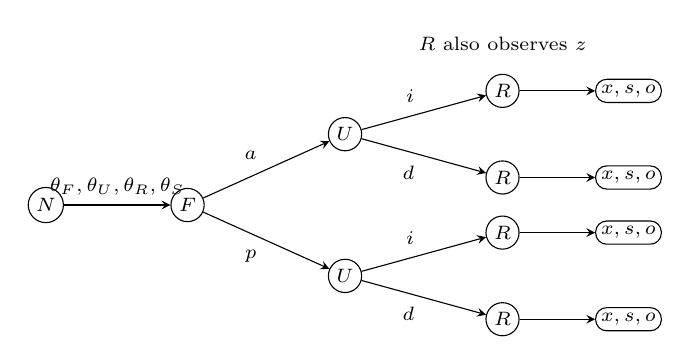
\begin{tikzpicture}[x=1cm,y=1cm,>=stealth,
  every node/.style={font=\scriptsize},
  decision/.style={circle,draw,inner sep=1.5pt},
  terminal/.style={rectangle,draw,rounded corners,inner sep=2pt}]
  \node[decision] (n) at (0,0) {$N$};
  \node[decision] (f) at (1.8,0) {$F$};
  \node[decision] (ua) at (3.8,0.9) {$U$};
  \node[decision] (up) at (3.8,-0.9) {$U$};
  \node[decision] (rai) at (5.8,1.45) {$R$};
  \node[decision] (rad) at (5.8,0.35) {$R$};
  \node[decision] (rpi) at (5.8,-0.35) {$R$};
  \node[decision] (rpd) at (5.8,-1.45) {$R$};
  \node[terminal] (tai) at (7.4,1.45) {$x,s,o$};
  \node[terminal] (tad) at (7.4,0.35) {$x,s,o$};
  \node[terminal] (tpi) at (7.4,-0.35) {$x,s,o$};
  \node[terminal] (tpd) at (7.4,-1.45) {$x,s,o$};
  \draw[->] (n) -- node[above] {$\theta_F,\theta_U,\theta_R,\theta_S$} (f);
  \draw[->] (f) -- node[above left] {$a$} (ua);
  \draw[->] (f) -- node[below left] {$p$} (up);
  \draw[->] (ua) -- node[above left] {$i$} (rai);
  \draw[->] (ua) -- node[below left] {$d$} (rad);
  \draw[->] (up) -- node[above left] {$i$} (rpi);
  \draw[->] (up) -- node[below left] {$d$} (rpd);
  \draw[->] (rai) -- (tai);
  \draw[->] (rad) -- (tad);
  \draw[->] (rpi) -- (tpi);
  \draw[->] (rpd) -- (tpd);
  \node at (5.8,2.05) {$R$ also observes $z$};
\end{tikzpicture}
\caption{Extensive-form skeleton of the signaling game. Nature draws private
types; $F$ signals first, $U$ responds, and $R$ acts after observing both public
messages and the noisy public signal $z$.}
\Description{A sequential signaling tree in which Nature draws types, the firm sends an anthropomorphic or deflationary message, the user invests or detaches, and the regulator inspects, sanctions, or abstains after also observing a public signal.}
\label{fig:signaling-tree}
\end{figure}

\subsection{Equilibrium Results}

\begin{proposition}[Profitable cheap-talk pooling]
\label{prop:pooling-pbe}
\label{thm:pooling}
Under Assumptions~\ref{ass:cheap-talk} and~\ref{ass:pooling}, pooling on anthropomorphic marketing is a Perfect Bayesian Equilibrium.  At $\rho_S=0$, the on-path anthropomorphic message has negative net signal cost for both governance types.
\end{proposition}
\begin{proof}
Consider the strategy profile where both firm types send $a$, both user types invest after $a$, and the regulator abstains.  Off path, users detach after $p$ and $R$ abstains.  Sequential rationality holds: a firm deviating to $p$ loses $\Delta_F^S$ because users detach, without reducing penalties because $R$ already abstains.  Users find investment optimal under the prior by Assumption~\ref{ass:pooling}.  Regulators abstain under the prior by Assumption~\ref{ass:pooling}.  Bayes consistency is satisfied because posteriors equal priors on path, and off-path beliefs are fixed at the prior.
\end{proof}

\begin{corollary}[Voluntary non-arbitrage is not incentive compatible]
\label{cor:voluntary-non-arbitrage}
For type $\theta$ in the pooling region, let $\mathbb{E}[P(m)]$ denote the expected penalty following message $m\in\{a,p\}$. If
\[
\Delta_F^S
>
c_\theta(a)-c_\theta(p)+\mathbb{E}[P(a)]-\mathbb{E}[P(p)],
\]
then choosing $a$ strictly dominates voluntary deflationary positioning $p$ for type $\theta$. Hence voluntary non-arbitrage is not incentive compatible.
\end{corollary}
\begin{proof}
In the pooling region, receiver beliefs and continuation behaviour are fixed as in Proposition~\ref{prop:pooling-pbe}. The payoff difference for type $\theta$ between choosing $a$ and choosing $p$ is
\[
u_\theta(a)-u_\theta(p)
=
\Delta_F^S-c_\theta(a)+c_\theta(p)-\mathbb{E}[P(a)]+\mathbb{E}[P(p)].
\]
The displayed hypothesis is exactly the condition that this difference is strictly positive. Therefore $a$ strictly dominates $p$, so unilateral voluntary refusal of the ontological premium is not a best response.
\end{proof}

\section{Shadowing and Neologism-Proofness: Why Trust-Restoring Signals Fail}
\label{sec:shadowing}

\begin{lemma}[Equal continuation premium under zero-cost mimicry]
\label{lem:equal-continuation}
Under Assumption~\ref{ass:cheap-talk}, the firm's payoff from any
trust-restoring continuation $c$ that induces user investment and regulatory
abstention is type-independent:
\[
u_\mathsf{H}(c)=u_\mathsf{L}(c)=\Delta_F^S .
\]
Therefore $u_\mathsf{H}(c)>\bar u_\mathsf{H}$ if and only if
$u_\mathsf{L}(c)>\bar u_\mathsf{L}$.
\end{lemma}
\begin{proof}
Under continuation $c$, the user invests ($m_U=i$) and the regulator abstains
($m_R=o$), so $P(m_R)=0$.  The firm's payoff is
$\Delta_F^S-c_{\theta_F}(a)-P(m_R)=\Delta_F^S-c_{\theta_F}(a)$.
Assumption~\ref{ass:cheap-talk} sets $c_\mathsf{H}(a)=c_\mathsf{L}(a)=0$,
so both types receive $\Delta_F^S$.  Since pooling-equilibrium payoffs
$\bar u_\mathsf{H}$ and $\bar u_\mathsf{L}$ are also type-independent under
Assumption~\ref{ass:cheap-talk} (both equal $\Delta_F^S$ from
Proposition~\ref{prop:pooling-pbe}), the strict-gain comparison reduces to
$\Delta_F^S>\bar u_\theta$ for both $\theta$ simultaneously.
\end{proof}

\begin{theorem}[Profitable shadowing at zero retaliation]
\label{thm:zero-retaliation-shadowing}
\label{thm:neologism}
When $\rho_S=0$, the pooling equilibrium of Proposition~\ref{prop:pooling-pbe} is neologism-proof against every nontrivial trust-restoring type claim: whenever a continuation is strictly profitable for the high-governance type, it is also shadowable by the low-governance type.
\end{theorem}
\begin{proof}
A neologism $K$ is credible only if the types in $K$ strictly prefer the induced continuation $c$, while types outside $K$ do not.  Take the only nontrivial trust-restoring claim, $K=\{\mathsf{H}\}$.  At $\rho_S=0$, the subject cannot impose any independent cost and $\Delta_F^S=\Delta_F$.  The continuation $c$ that restores trust induces user investment and regulatory abstention.  By Lemma~\ref{lem:equal-continuation}, the firm's payoff under $c$ is type-independent: $u_\mathsf{H}(c)=u_\mathsf{L}(c)=\Delta_F^S$.  Therefore
\[
u_\mathsf{H}(c)>\bar u_\mathsf{H}
\quad\Longrightarrow\quad
u_\mathsf{L}(c)>\bar u_\mathsf{L},
\]
so the deviation cannot exclude $\mathsf{L}$.  The trust-restoring neologism is not credible in Farrell's sense.
\end{proof}

The point is not that the low-governance type is merely able to mimic.  Whenever the continuation premium exceeds expected penalty, mimicry is itself the low-governance type's best response.  Trust-restoring neologisms therefore fail before they can make governance quality common knowledge: the message that would form common knowledge is profitably shadowable.

\begin{corollary}[Zero-retaliation boundary]
\label{cor:retaliation-boundary}
\label{thm:comparative}
Let the effective premium be $\Delta_F^S = \Delta_F - \rho_S C_S$, where $\rho_S \in [0,1]$ is the subject's retaliation capacity and $C_S$ is the cost imposed through resistance, exit, litigation, or sanction.  The boundary $\rho_S=0$ removes this constraint class and leaves the premium unconstrained by subject retaliation.
\end{corollary}
\begin{proof}
When $\rho_S>0$, the subject can impose expected cost $\rho_SC_S$, shrinking the pooling region.  When $\rho_S=0$, $\Delta_F^S=\Delta_F$, so the off-equilibrium punishment path disappears.
\end{proof}

\begin{remark}[Agentic systems and $\rho_S$]
The model distinguishes causal capacity from payoff-imposing capacity. Tool use is not retaliation. The parameter $\rho_S$ does not measure whether an AI system can send emails, post messages, call tools, or coordinate activity through firm-provided affordances. It measures whether the classified object can impose an independent cost on the sender's classification of it. Agentic AI may increase public visibility, detection probability, or regulator bandwidth, thereby changing $z$, $K_R$, $D_R$, or expected penalties. But unless the system has a protected and non-waivable channel of refusal, exit, sanction, litigation, or cost-imposition, its subject-retaliation capacity remains zero. A future regime that grants such a channel is covered by the comparative statics $\Delta_F^S=\Delta_F-\rho_S C_S$; the zero-retaliation case studied here is the limit in which behavioral agency does not yet amount to strategic standing.
\end{remark}

\subsection{Robustness of Off-Path Beliefs}
\label{subsec:robustness}

A standard critique of pooling equilibria is their reliance on particular off-path beliefs. In Theorem~\ref{thm:pooling}, off-path beliefs are fixed at the prior, and the user detaches after observing a deviation to $p$. One might argue that the equilibrium would collapse under stronger refinement concepts. We show that any off-path belief assigning credibility to a high-governance deviation is defeated by $\mathsf{L}$-type mimicry. 

If a receiver assigns a high posterior to $\mathsf{H}$ following an out-of-equilibrium message $m'$, the message induces user investment. But because signaling costs are zero (Assumption~\ref{ass:cheap-talk}), the $\mathsf{L}$-type firm can trivially imitate $m'$. Since $\Delta_F^S$ is captured uniformly, the $\mathsf{L}$-type strict deviation payoff strictly exceeds its pooling payoff whenever the $\mathsf{H}$-type deviation payoff does. 

Consequently, standard type-exclusion refinements like the Intuitive Criterion \citep{cho_kreps1987} and Divinity \citep{banks_sobel1987} do not select the desired separating deviation. The Intuitive Criterion eliminates types for whom the deviation is equilibrium-dominated regardless of the receiver's best response. Here, neither type is equilibrium-dominated because both types strictly benefit if the receiver invests. Farrell's neologism-proofness \citep{farrell1993} therefore becomes the mathematically appropriate refinement: it asks whether a message with a literal meaning can be believed. As Theorem~\ref{thm:neologism} shows, the zero-retaliation limit ensures perfect shadowing, meaning no such belief can be sustained in equilibrium. The pathology is not that off-path beliefs are too weak, but that any trust-restoring belief is immediately devoured by shadowing.

% !TEX root = ../arbitrage.tex
\section{Cost-Imposed Separation: How Common Knowledge Becomes Possible}
\label{sec:cheap-talk}

Separation is not moral communication.  It is engineered common-knowledge formation through externally imposed signal costs.  In the baseline, $a$ is profitable cheap talk because $\operatorname{NetCost}_{\theta}(a)<0$ for both governance types.  An audit requirement changes the message space and asks whether the trust-restoring signal can be priced so that the high-governance type can still send it while the low-governance type cannot profitably shadow it.

\begin{theorem}[Cost-imposed common-knowledge formation]
\label{thm:audit-cost-separation}
\label{thm:separation}
Consider the audit-augmented message space
\[
M_F^e=\{p,a_0\}\cup\{\widehat a(e):e\geq0\},
\]
where $p$ is deflationary positioning, $a_0$ is an unaudited anthropomorphic
claim, and $\widehat a(e)$ is an anthropomorphic claim accompanied by an audit
trail of intensity $e$.  Let $G$ denote the gross continuation gain to the firm
from having $\widehat a(e)$ accepted as credible, before paying the audit cost.
Equivalently, $G$ is the trust-restoration premium: in the benchmark payoff
normalization above $G=\Delta_F^S$, while if audit acceptance also changes the
regulator's continuation from inspection or sanction to abstention, $G$ includes
the avoided expected penalty.  Under an audit-trail signal cost satisfying the
single-crossing condition
\[
c_\mathsf{H}(e,\theta_S)\leq G\leq c_\mathsf{L}(e,\theta_S),
\]
a separating Perfect Bayesian Equilibrium exists.
\end{theorem}
\begin{proof}
Let $c_\theta(e,\theta_S)=k_\theta e+\theta_S$, with $0<k_H<k_L$.  For an audit intensity
\[
e\in\left[\frac{G-\theta_S}{k_L},\frac{G-\theta_S}{k_H}\right],
\]
the high-governance type prefers the audited anthropomorphic signal
$\widehat a(e)$, netting $G-c_\mathsf{H}(e,\theta_S)\geq0$, while the
low-governance type does not mimic because
$G-c_\mathsf{L}(e,\theta_S)\leq0$.  Beliefs assign $\mathsf{H}$ to
$\widehat a(e)$ and $\mathsf{L}$ to the deflationary signal.  The unaudited
claim $a_0$ receives the same posterior treatment as profitable cheap talk and therefore
does not produce the trust-restoring continuation $G$.  Given these beliefs,
user investment and regulatory abstention after $\widehat a(e)$, and detachment
or inspection after non-audited signals, are sequentially rational in the
separating region.
\end{proof}

The theorem is the Spence step in the paper.  A trust-restoring signal becomes credible only when the external cost schedule reverses the negative net cost of the baseline signal and satisfies single crossing.  The high type must face
\[
\operatorname{NetCost}_{\mathsf{H}}(\widehat a(e))
=
c_\mathsf{H}(e,\theta_S)-G
\leq0,
\]
while the low type must face
\[
\operatorname{NetCost}_{\mathsf{L}}(\widehat a(e))
=
c_\mathsf{L}(e,\theta_S)-G
\geq0.
\]
Only then can the audited signal support common-knowledge formation rather than another shadowable message.

Theorem~\ref{thm:audit-cost-separation} gives the local separation condition.
The mechanism consequences---sanctionable inconsistency, audit requirements,
and auditable records---are stated as
Corollaries~\ref{cor:inconsistency-pruning}--\ref{cor:verification-feasibility}
in Section~\ref{sec:mechanism} after introducing a common notation for
the low-type arbitrage spread.  That notation is useful because the three
interventions operate on different terms of the same net-payoff inequality.

\section{Why Profitable Cheap Talk Does Not Self-Correct}
\label{sec:persistence}

Theorem~\ref{thm:audit-cost-separation} identifies the cost condition that restores separation.  This section explains why profitable cheap talk persists when that condition is absent.  Each persistence mechanism is matched to a parameter of the model so that the proposals in Section~\ref{sec:mechanism} can be read as targeted cost changes rather than as welfare exhortations. They preserve negative net signal cost or prevent the penalty term from exceeding the premium.

\emph{Opacity.} The system-opacity parameter $\theta_S$ is private to the firm. Capability claims about a deployed model cannot be falsified by reading model outputs alone, because the same outputs are compatible with very different training procedures, evaluation regimes, and post-deployment monitoring. Opacity is the precondition for the firm's premium: where outsiders could costlessly verify $\theta_F$, the spread between anthropomorphic and deflationary positioning would collapse. This is the lemons logic of \citet{akerlof1970}: under one-sided private information, the market clears at a price that reflects the worst credible quality, except that here the relevant ``quality'' is a governance disposition rather than a physical attribute.

\emph{Verification bandwidth.} The third inequality of the pooling region, $K_{\theta_R}>\pi(\mathsf{L})D_R$, encodes the regulator's inspection cost relative to expected gain. A low-bandwidth regulator faces an absolute cost so high that abstention is dominant under the prior; even a high-bandwidth regulator may be priced out across the full product population. The condition that produces this state is not unique to AI. \citet{pasquale2015} documents the same inspection-cost architecture in algorithmic finance and consumer scoring: the opacity of the regulated object combines with the bandwidth of the regulator to make inspection a scarce resource allocated by triage rather than by uniform application.

\emph{Asynchronous harms.} The user's payoff term $H_{\theta_U}$ enters discounted. The episodes in which a relational reading proves costly---deprecation, persona shifts, crisis-handling failures---are temporally separated from the initial attribution by intervals over which the user has already accrued $B_{\theta_U}$. Under standard hyperbolic or even exponential discounting, the inequality $B_{\theta_U}-\pi(\mathsf{L})H_{\theta_U}>0$ holds for a wider class of users than the time-zero risk calculation would suggest. Asynchrony is not a behavioural bug; it is the timing structure of the harm itself.

\emph{Fragmentation of affected parties.} Publics, journalists, intellectuals, and affected communities are folded into the noisy channel $z$ rather than modelled as autonomous players. This is not a normative claim that they lack standing; it is an institutional observation. Their costs of coordination are high, their access to inspection technology is uneven, and their incentives to invest in any particular case are individually small. Even when $z$ carries substantial information about $\theta_F$, regulators cannot treat it as binding without a procedural translation that the channel itself does not provide. The fragmentation result is closely related to the cheap-talk multiplicity of \citet{crawford_sobel1982}: with many would-be senders and a single noisy aggregator, the informative subset of equilibria is not selected for.

\emph{No penalty for inconsistency.} The profitable cheap-talk cost structure sets $c_{\theta_F}(a)=c_{\theta_F}(p)=0$ for both governance types and---more importantly for this section---imposes no joint constraint across $m_F$. Marketing copy and policy documentation are produced under different audiences, different review processes, and different liability regimes. Inconsistency between them is not detected as a single offence; it is decomposed into two compliant statements at two different points of contact. The firm's premium $\Delta_F$ is rent earned precisely on this decomposition. Until the signal cost makes inconsistency itself sanctionable---the proposal of Section~\ref{subsec:sanctionable-inconsistency}---there is no parameter under the firm's control whose adjustment would close the spread.

\emph{Pooling is the stable outcome selected by the current incentive structure.} These five structural conditions jointly explain why normative declarations do not change equilibrium behavior unless they alter the signal-cost structure. The constraint is not a failure of moral seriousness, but a formal property of the message space: a declaration of ``responsible AI'' is indistinguishable from any other message at $c_{\theta_F}(a)=0$ while $\operatorname{NetCost}_{\theta}(a)<0$. Because both governance types can issue it at the same cost and capture the same premium, it contains no type information and moves no posterior. The pooling outcome is therefore the stable equilibrium of the incentive structure as currently constituted, even if it is welfare-reducing in aggregate. A firm that unilaterally forgoes the ontological premium $\Delta_F$---that chooses deflationary marketing across all channels and forfeits the user investment it would otherwise attract---loses revenue it cannot recover from customers who face no such constraint. The implication is precise: within the pooling region defined above, unilateral non-arbitrage is not a best response; a firm that forgoes $\Delta_F$ loses the induced investment while competitors retain it. The mechanisms in Section~\ref{sec:mechanism} respond to this implication by changing the cost parameters rather than appealing to the conscience of players who are already acting rationally.

\begin{table}[ht]
\centering
\small
\setlength{\tabcolsep}{4pt}
\begin{tabular}{@{}lll@{}}
\toprule
\textbf{Structural Condition} & \textbf{Model Parameter} & \textbf{Intervention (\S\ref{sec:mechanism})} \\
\midrule
No penalty for inconsistency & $\operatorname{NetCost}_{\theta}(a)<0$ & Sanctionable inconsistency \\
Opacity & $\theta_S$ private to firm & Costly third-party audits \\
Verification bandwidth & $K_{\theta_R}>\pi(\mathsf{L})D_R$ & Auditable records \\
Asynchronous harms & $H_{\theta_U}$ enters discounted & Evidentiary lag priced \\
Fragmentation & $z$ noisy, high coord.\ cost & Aggregation cost lowered \\
\bottomrule
\end{tabular}
\caption{Mapping of structural persistence conditions to model parameters and cost-imposition mechanisms.}
\label{tab:condition-map}
\end{table}

% !TEX root = ../arbitrage.tex
\section{Endogenous Trust Dynamics}
\label{sec:trust-dynamics}

The dynamic question is whether repeated interaction, user habituation, and
delayed harms can substitute for externally priced signals.  They cannot do so
merely by adding history to the baseline game.  The zero-retaliation boundary
continues to matter dynamically because the anthropomorphic message expands
the trust stock without imposing a corresponding production, verification, or
sanction cost on the sender.

\subsection{The Law of Motion for Endogenous Trust}
\label{subsec:trust-law}

Embed the baseline setting into an infinite-horizon Markov game.  Let the
public state variable $x_t\in X\subseteq\mathbb R_+$ denote endogenous trust
capital, or relational reliance, accumulated in the user base at the beginning
of period $t$.  The state evolves according to
\[
x_{t+1}
=
\alpha x_t+\beta i_t+\gamma\mathbf 1_{\{m_t=a\}}-\delta q_t .
\]
The state variable $x_t$ is the aggregate stock of structural and affective
reliance users place in the system.  The firm's stage-game ontological premium
and the user's baseline utility from investment are strictly increasing in
$x_t$.  The parameter $\alpha\in(0,1)$ is trust persistence; $1-\alpha$ is the
natural depreciation of user trust in the absence of continued engagement or
new trust-restoring messages.  The action $i_t\in\{0,1\}$ is user investment:
$i_t=1$ denotes investment, and $i_t=0$ denotes detachment.  The coefficient
$\beta\ge0$ is habituation or engagement reinforcement, so active user
investment raises the next-period reliance baseline.

The indicator $\mathbf 1_{\{m_t=a\}}$ equals one when the firm sends the
trust-restoring anthropomorphic message and zero under deflationary
positioning.  The coefficient $\gamma>0$ is the costless semantic premium: the
deterministic expansion of trust capital generated by the anthropomorphic
signal.  Because the zero-retaliation boundary sets $c_\theta(a)=0$, this
state expansion is not matched by a production or verification cost.  The shock
$q_t\ge0$ is asynchronous harm realization, drawn from
$F(\cdot\mid\theta_F)$, with
\[
\mathbb E[q_t\mid\theta_F=L]>\mathbb E[q_t\mid\theta_F=H].
\]
It represents delayed leakage of private governance type through capability
deprecation, unannounced persona shifts, abrupt refusals, or related adverse
incidents.  The parameter $\delta>0$ is the depletion penalty per unit of
asynchronous harm.

\begin{theorem}[Almost-Sure Dynamic Pooling Invariance]
\label{thm:dynamic-pooling-invariance}
Let the endogenous trust state evolve according to
\[
x_{t+1}
=
\alpha x_t+\beta i_t+\gamma\mathbf 1_{\{m_t=a\}}-\delta q_t,
\]
where $\alpha\in(0,1)$, $\beta\ge 0$, $\gamma>0$, and $\delta>0$.
For each governance type $\theta\in\{H,L\}$, let
\[
\operatorname{supp}(q_t\mid \theta)\subseteq [0,\bar q_\theta],
\]
with $\bar q_L>\bar q_H\ge 0$.

Let $I=[\underline x,\bar x]\subseteq \mathbb R_+$.
Suppose that the semantic premium and habituation reinforcement satisfy
\[
(1-\alpha)\underline{x}+\delta\bar q_L
\le
\beta+\gamma
\le
(1-\alpha)\bar{x}.
\]
Suppose further that, for every $x\in I$, users strictly prefer investment
after the anthropomorphic message under the pooling belief, and both firm
types satisfy the Bellman incentive constraint for sending $a$ rather than
any alternative message.

Then there exists a Markov perfect pooling equilibrium on $I$ in which both
types send $a$, users invest, and the interval $I$ is almost surely
forward-invariant. That is, for every $x_t\in I$,
\[
\mathbb P
\left(
\alpha x_t+\beta+\gamma-\delta q_t\in I
\;\middle|\;
x_t\in I
\right)
=
1.
\]
Consequently, along this equilibrium path, the trust state never escapes
$I$ despite recurring asynchronous harms.
\end{theorem}
\begin{proof}
Under the pooling profile, $m_t=a$ and $i_t=1$, so
\[
x_{t+1}
=
\alpha x_t+\beta+\gamma-\delta q_t.
\]
For any $x_t\in I$ and any $q_t\in[0,\bar q_L]$, the transition is minimized
at $x_t=\underline x$ and $q_t=\bar q_L$. Hence
\[
x_{t+1}
\ge
\alpha\underline x+\beta+\gamma-\delta\bar q_L
\ge
\underline x
\]
by the lower-bound condition. The transition is maximized at
$x_t=\bar x$ and $q_t=0$. Hence
\[
x_{t+1}
\le
\alpha\bar x+\beta+\gamma
\le
\bar x
\]
by the upper-bound condition. Therefore
\[
x_{t+1}\in[\underline x,\bar x]=I
\]
for every feasible shock realization. Since
$\operatorname{supp}(q_t\mid\theta)\subseteq[0,\bar q_\theta]$ and
$\bar q_H<\bar q_L$, the same bound applies to both types. Thus $I$ is
forward-invariant almost surely.

The assumed user optimality and Bellman incentive constraints support the
pooling Markov strategy profile on $I$. Therefore the invariant pooling path
is a Markov perfect pooling equilibrium.
\end{proof}

The logic is the dynamic counterpart of profitable cheap talk:
\[
\gamma+\beta
\quad\text{sustain the trust stock,}
\]
\[
\Rightarrow\quad
\text{pooling remains dynamically invariant.}
\]
The next issue is therefore not whether history exists, but whether history is
priced.  If a reputation or repair message remains costless at the
zero-retaliation boundary, it is another trust-restoring signal available to
the low-governance type.  Dynamic separation requires a priced wedge: audit,
certification, sanctionable inconsistency, or another mechanism that changes
the Bellman value comparison rather than merely adding an unpriced history
variable.

\subsection{Dynamic Shadowing and No Trust-Restoring History}
\label{subsec:dynamic-shadowing}

The dynamic environment reverses the Spence logic.  In a standard
costly-signaling model, the high type values separation more because it can
bear the signal cost more cheaply.  Here, at the zero-retaliation boundary, the
signal is unpriced.  Since the low-governance type loses trust faster on the
pooling path, a free trust-restoring message creates at least as large a net
continuation gain for the low type as for the high type.  The deviation is
therefore shadowed rather than separating.

\begin{theorem}[Dynamic Shadowing and Endogenous Reverse Single-Crossing]
\label{thm:dynamic-shadowing}
Let $\bar{V}_\theta(x_t)$ denote the continuation value of type
$\theta\in\{H,L\}$ on the almost-sure pooling path at state $x_t\in I$.
Suppose a high-governance firm attempts to break the pooling equilibrium by
issuing an unpriced, history-dependent trust-restoring neologism $c(h_t)$.
Let $V_\theta(c,x_t)$ denote the continuation value of type $\theta$ if
receivers accept the message as credible.

A dynamically credible separating deviation requires
\[
V_H(c,x_t)-\bar{V}_H(x_t)>0
\]
and
\[
V_L(c,x_t)-\bar{V}_L(x_t)\le 0.
\]

At the zero-retaliation boundary, the message $c(h_t)$ imposes no
type-differential execution cost.  Moreover, because the low-governance type
faces stochastically larger asynchronous harms on the pooling path, its
pooling continuation value is weakly lower:
\[
\bar{V}_L(x_t)\le \bar{V}_H(x_t).
\]
Assume further that the accepted neologism weakly compresses the
type-continuation wedge:
\[
V_H(c,x_t)-V_L(c,x_t)
\le
\bar{V}_H(x_t)-\bar{V}_L(x_t).
\]
Then the net continuation premium satisfies the reverse single-crossing
inequality
\[
V_L(c,x_t)-\bar{V}_L(x_t)
\ge
V_H(c,x_t)-\bar{V}_H(x_t).
\]
Consequently, if the neologism is strictly profitable for the high type,
\[
V_H(c,x_t)-\bar{V}_H(x_t)>0,
\]
then it is also strictly profitable for the low type:
\[
V_L(c,x_t)-\bar{V}_L(x_t)>0.
\]
Thus every profitable unpriced trust-restoring neologism is dynamically
shadowed by the low-governance type and cannot sustain type separation.
\end{theorem}
\begin{proof}
The wedge-compression condition gives
\[
V_H(c,x_t)-V_L(c,x_t)
\le
\bar{V}_H(x_t)-\bar{V}_L(x_t).
\]
Rearranging yields
\[
V_L(c,x_t)-\bar{V}_L(x_t)
\ge
V_H(c,x_t)-\bar{V}_H(x_t).
\]
Hence, whenever
\[
V_H(c,x_t)-\bar{V}_H(x_t)>0,
\]
we also have
\[
V_L(c,x_t)-\bar{V}_L(x_t)>0.
\]
The low-governance type therefore strictly benefits from issuing the same
history-dependent neologism. The deviation cannot be assigned exclusively to
the high-governance type under any credible separating belief. Therefore the
unpriced trust-restoring message is dynamically shadowed.
\end{proof}

\begin{corollary}[Symmetric Trust Reset]
\label{cor:symmetric-trust-reset}
If an accepted trust-restoring neologism resets the receiver-facing trust state
symmetrically so that
\[
V_L(c,x_t)=V_H(c,x_t),
\]
then the wedge-compression condition holds automatically whenever
\[
\bar{V}_L(x_t)\le \bar{V}_H(x_t).
\]
Thus every profitable high-type neologism is strictly shadowed by the low type.
\end{corollary}
\begin{proof}
If $V_L(c,x_t)=V_H(c,x_t)$, then
\[
V_H(c,x_t)-V_L(c,x_t)=0.
\]
The condition $\bar{V}_L(x_t)\le \bar{V}_H(x_t)$ gives
\[
0\le \bar{V}_H(x_t)-\bar{V}_L(x_t),
\]
which is exactly the wedge-compression condition.  The shadowing conclusion
then follows from Theorem~\ref{thm:dynamic-shadowing}.
\end{proof}

\subsection{Externally Priced Dynamic Separation}
\label{subsec:dynamic-separation}

The dynamic Spence ratio shows why the standard costly-signaling intuition is
incomplete in endogenous trust environments.  It is not enough that the
low-governance type faces a higher marginal audit cost.  Because the low type
also receives a larger dynamic premium from escaping the deteriorating pooling
path, the audit technology must discriminate faster than the endogenous
continuation premium grows.  Separation requires not merely $c_L>c_H$, but
\[
\frac{c_L}{c_H}>
\frac{\Delta V_L}{\Delta V_H}.
\]

\begin{theorem}[Externally Priced Separation via Dynamic Single-Crossing]
\label{thm:externally-priced-dynamic-separation}
Consider the almost-sure pooling regime supported on the invariant trust
interval $I$. Let an external mechanism make available a verifiable signal
$s$ with type- and state-dependent cost $k_\theta(s,x)$, where
$\theta\in\{H,L\}$.

Let $V_\theta^S(x)$ denote the before-cost expected continuation value of
successfully separating and securing the relational premium, and let
$V_\theta^P(x)$ denote the continuation value of remaining on the unverified
pooling path. Define
\[
\Delta V_\theta(x)
:=
V_\theta^S(x)-V_\theta^P(x).
\]

Within the class of audit-supported Markov equilibria, the signal $s$
supports a separating Markov perfect equilibrium on $I$ if and only if, for
every $x\in I$,
\[
k_L(s,x)>\Delta V_L(x)
\]
and
\[
k_H(s,x)\le \Delta V_H(x).
\]
The first inequality deters the low-governance type from mimicking the
separating signal; the second gives the high-governance type a weakly
profitable incentive to separate.
\end{theorem}
\begin{proof}
At state $x$, the low-governance type's net gain from mimicking the
separating signal is
\[
\Delta V_L(x)-k_L(s,x).
\]
The low type is deterred precisely when this quantity is strictly negative,
equivalently $k_L(s,x)>\Delta V_L(x)$.  The high-governance type's net gain
from sending the separating signal is
\[
\Delta V_H(x)-k_H(s,x).
\]
The high type weakly prefers separation precisely when this quantity is
nonnegative, equivalently $k_H(s,x)\le\Delta V_H(x)$.  These two incentive
constraints are necessary for a separating Markov equilibrium supported by
the audit signal, and, within the stated class of audit-supported Markov
equilibria, they are sufficient: assign $s$ to the high type, assign the
unverified pooling action to the low type, and let receivers treat the
verified signal as credible.
\end{proof}

\begin{remark}[Structural wedge]
\label{rem:dynamic-structural-wedge}
Recall from Theorem~\ref{thm:dynamic-shadowing} that unpriced semantic claims
yield an endogenous reverse single-crossing: $\Delta V_L(x)\ge\Delta V_H(x)$.
A necessary implication of the two inequalities in
Theorem~\ref{thm:externally-priced-dynamic-separation} is
\[
k_L(s,x)-k_H(s,x)
>
\Delta V_L(x)-\Delta V_H(x)\ge 0.
\]
Thus the external mechanism must generate a cost wedge large enough to
overpower the low type's endogenous trust-reset advantage.
\end{remark}

\begin{corollary}[Separating Audit Intensity and the Dynamic Spence Ratio]
\label{cor:dynamic-spence-ratio}
Suppose the external mechanism is parameterized by a scalar audit intensity
$e\ge 0$, with linear type-dependent costs
\[
k_\theta(e,x)=c_\theta(x)e,
\]
where
\[
c_L(x)>c_H(x)>0.
\]
Assume further that
\[
\Delta V_L(x)\ge \Delta V_H(x)>0.
\]

A state-contingent audit intensity $e^*(x)$ supporting separation at state
$x$ exists if and only if
\[
\frac{c_L(x)}{c_H(x)}
>
\frac{\Delta V_L(x)}{\Delta V_H(x)}
\ge 1.
\]
When this ratio condition holds, any audit intensity satisfying
\[
e^*(x)\in
\left(
\frac{\Delta V_L(x)}{c_L(x)},
\frac{\Delta V_H(x)}{c_H(x)}
\right]
\]
supports separation at state $x$. If the ratio condition fails, the
separating interval is empty, and every audit intensity affordable to the
high-governance type is also profitably shadowed by the low-governance type.
\end{corollary}
\begin{proof}
By Theorem~\ref{thm:externally-priced-dynamic-separation}, separation at
state $x$ requires
\[
c_L(x)e>\Delta V_L(x)
\qquad\text{and}\qquad
c_H(x)e\le\Delta V_H(x).
\]
Since $c_L(x)>c_H(x)>0$, this is equivalent to
\[
e>
\frac{\Delta V_L(x)}{c_L(x)}
\qquad\text{and}\qquad
e\le
\frac{\Delta V_H(x)}{c_H(x)}.
\]
The feasible interval is nonempty if and only if
\[
\frac{\Delta V_L(x)}{c_L(x)}
<
\frac{\Delta V_H(x)}{c_H(x)},
\]
which, because $\Delta V_H(x)>0$ and $c_H(x)>0$, is equivalent to
\[
\frac{c_L(x)}{c_H(x)}
>
\frac{\Delta V_L(x)}{\Delta V_H(x)}.
\]
The lower bound $\Delta V_L(x)/\Delta V_H(x)\ge1$ follows from the assumed
reverse dynamic premium.
\end{proof}

\begin{corollary}[Uniform Audit Intensity]
\label{cor:uniform-audit-intensity}
A single audit intensity $e$ supports separation throughout the interval $I$
if and only if
\[
\sup_{x\in I}
\frac{\Delta V_L(x)}{c_L(x)}
<
\inf_{x\in I}
\frac{\Delta V_H(x)}{c_H(x)}.
\]
In that case, any
\[
e\in
\left(
\sup_{x\in I}\frac{\Delta V_L(x)}{c_L(x)},
\inf_{x\in I}\frac{\Delta V_H(x)}{c_H(x)}
\right]
\]
supports a separating Markov equilibrium on $I$.
\end{corollary}
\begin{proof}
For a fixed $e$ to support separation at every $x\in I$, it must satisfy
\[
e>
\frac{\Delta V_L(x)}{c_L(x)}
\qquad\text{and}\qquad
e\le
\frac{\Delta V_H(x)}{c_H(x)}
\]
for every $x\in I$.  This is equivalent to
\[
e>
\sup_{x\in I}
\frac{\Delta V_L(x)}{c_L(x)}
\qquad\text{and}\qquad
e\le
\inf_{x\in I}
\frac{\Delta V_H(x)}{c_H(x)}.
\]
Such an $e$ exists if and only if the displayed strict inequality between the
supremum and infimum holds.
\end{proof}

This corollary separates pointwise mechanism design from institutional design:
\[
\text{local audit feasibility}
\neq
\text{uniform institutional feasibility}.
\]
An audit technology can separate types at each isolated state while still
failing to provide a single administrable intensity that works across the
entire trust interval.
% !TEX root = ../arbitrage.tex
\section{Pricing the Ontological Spread: Necessity and Sufficiency Conditions}
\label{sec:mechanism}

The three interventions below are an external pricing architecture.  The
section moves from formal model to mechanism implication to institutional
implementation:
\[
\text{formal model}
\to
\text{mechanism implication}
\to
\text{institutional implementation}.
\]
Sanctionable inconsistency prices the cross-channel spread.  Audits price the
anthropomorphic claim.  Auditable records price verification by changing the
regulator's inspection inequality.  The mechanisms therefore operate on
different margins of the same zero-retaliation arbitrage condition.

\begin{definition}[Low-type arbitrage spread]
\label{def:arbitrage-spread}
Define the low-type arbitrage spread from a trust-restoring register $q$ as
\[
\Omega_L(q)
  := G(q)-C_L(q)-\Pi_L(q),
\]
where $G(q)$ is the gross continuation gain from the register,
$C_L(q)$ is the low type's signal or compliance cost, and
$\Pi_L(q)$ is the expected enforcement price attached to that register.
A low-governance type profitably shadows whenever $\Omega_L(q)>0$.
A mechanism disciplines profitable cheap talk only if it drives
$\Omega_L(q)\le 0$ while preserving $\Omega_H(q)\ge 0$ for the desired
high-governance signal.
\end{definition}

\begin{proposition}[Pricing the ontological spread]
\label{prop:pricing}
Let $q$ be a trust-restoring register or claim.  In the profitable cheap-talk
baseline, $C_H(q)=C_L(q)=0$ and $\Pi_H(q)=\Pi_L(q)=0$, so
\[
\Omega_H(q)=\Omega_L(q)=G(q)>0.
\]
Thus $q$ cannot separate types.  A mechanism can restore separation or prune
arbitrage only by altering at least one of three terms:
\[
\Omega_\theta(q)=G(q)-C_\theta(q)-\Pi_\theta(q).
\]

\emph{(i)} A sanctionable-inconsistency rule raises $\Pi_L(q)$ for inconsistent
cross-channel registers.

\emph{(ii)} An audit requirement raises $C_\theta(q)$ in a type-dependent way.

\emph{(iii)} Auditable records raise the probability or payoff of enforcement by
lowering $K_R$, increasing $D_R$, or increasing the detection probability
embedded in $\Pi_\theta(q)$.

\noindent
For a separating trust-restoring signal to exist, it is necessary that some
mechanism create a wedge such that
\[
\Omega_H(q)\ge 0 \quad \text{and} \quad \Omega_L(q)\le 0.
\]
Absent such a wedge, every trust-restoring message remains shadowable.
Within the audit family $c_\theta(e,\theta_S)=k_\theta e+\theta_S$,
the single-crossing condition
\[
c_H(e,\theta_S)\le G(q)\le c_L(e,\theta_S)
\]
is necessary and sufficient for separation by audit intensity.
\end{proposition}

\begin{remark}[Scope of the exhaustiveness claim]
\label{rem:three-terms-scope}
The claim that a mechanism can operate \emph{only} through $G$, $C_\theta$, or
$\Pi_\theta$ is exhaustive within the single-shot baseline of
Section~\ref{sec:bayesian}, where payoffs are stage-game quantities and
$\Omega_\theta(q)$ is defined over a single interaction.  In dynamic or
multi-product extensions, reputation effects may lower the effective premium
$G$ through adverse posteriors that persist across periods, and multi-product
cost spillovers may raise $C_\theta$ as a by-product of compliance
investments elsewhere in the firm's portfolio.  Either channel could
discipline the pooling equilibrium without an explicit external instrument.
Those extensions are consistent with the pricing proposition; they
instantiate it by altering $G$ and $C_\theta$ through endogenous market
forces rather than regulatory mandates.  The present paper establishes
conditions under which such endogenous forces are absent and external
cost-imposition is necessary---the zero-retaliation, no-reputation,
single-product limit studied in Sections~\ref{sec:three-sided}--\ref{sec:persistence}.
\end{remark}

\begin{corollary}[Sufficiency of sanctionable inconsistency for register pruning]
\label{cor:inconsistency-pruning}
For an inconsistent cross-channel register $q=(a,p)$, a
penalty for sanctionable inconsistency prunes the register whenever
\[
\rho_R SI \ge \Delta_F^S.
\]
If $\rho_R SI=0$ and no other mechanism prices inconsistency, then $q$
remains profitable whenever $\Delta_F^S>0$.
\end{corollary}

\begin{corollary}[Necessary and sufficient audit condition]
\label{cor:audit-separation}
Within the audit family $c_\theta(e,\theta_S)=k_\theta e+\theta_S$ with
$0<k_H<k_L$, an audited anthropomorphic signal supports separation if and
only if there exists $e\ge 0$ such that
\[
c_H(e,\theta_S)\le G\le c_L(e,\theta_S).
\]
Equivalently, when $G>\theta_S$,
\[
e\in
\left[
\frac{G-\theta_S}{k_L},\;
\frac{G-\theta_S}{k_H}
\right].
\]
\end{corollary}

\begin{corollary}[Verification feasibility]
\label{cor:verification-feasibility}
Auditable records make active regulation sequentially rational whenever
\[
K_R-\lambda \le \pi(\mathsf{L})(D_R+\eta).
\]
If this inequality fails, recordkeeping alone does not discipline profitable
cheap talk; it stores information without making enforcement
incentive-compatible.
\end{corollary}

\begin{table}[t]
\centering
\footnotesize
\setlength{\tabcolsep}{3pt}
\renewcommand{\arraystretch}{1.3}
\begin{tabular}{@{}p{2.6cm}p{2.6cm}p{2.9cm}p{2.9cm}@{}}
\toprule
\textbf{Mechanism} & \textbf{Prices what?} & \textbf{Sufficient for} & \textbf{Necessary when} \\
\midrule
Sanctionable inconsistency & cross-channel spread $(a,p)$ & pruning inconsistent register if $\rho_R SI\ge\Delta_F^S$ & no other mechanism prices inconsistency \\
Costly audit & anthropomorphic claim $a$ & type separation if $c_H\le G\le c_L$ & separation by message requires type-dependent cost wedge \\
Auditable records & verification / enforcement feasibility & inspection if $K_R{-}\lambda\le\pi(\mathsf{L})(D_R{+}\eta)$ & detection probability or verification payoff remains too low \\
\bottomrule
\end{tabular}
\caption{Mechanism matrix: each intervention prices a different margin of the
arbitrage spread $\Omega_\theta(q)$.}
\label{tab:mechanism-matrix}
\end{table}

\begin{table}[t]
\centering
\footnotesize
\setlength{\tabcolsep}{3pt}
\renewcommand{\arraystretch}{1.2}
\begin{tabular}{@{}p{3.0cm}p{3.0cm}p{4.3cm}@{}}
\toprule
Mechanism & Model term priced & Institutional form \\
\midrule
Sanctionable inconsistency & $(a,p)$ register spread & net-impression / substantiation review \\
Costly audit & $k_\theta(s,x)$ & substantiation-before-reliance \\
Auditable records & $K_R, D_R$ & record-backed oversight \\
\bottomrule
\end{tabular}
\caption{Institutional forms of external pricing.}
\label{tab:institutional-pricing}
\end{table}

\paragraph{Complementarity.}
The mechanisms are not substitutes.  They price different margins.
Sanctionable inconsistency without records imposes a penalty that the regulator
cannot verify---a paper tiger when $\rho_R$ is low.  Records without
sanctionable inconsistency store information without attaching a price:
an archive, not a mechanism.  Audit requirements without sanctionable
inconsistency can support a verified $(a,a)$ claim, but cannot automatically
prohibit the cross-channel $(a,p)$ arbitrage register.  Sanctionable
inconsistency combined with records prunes inconsistent registers.  Audit
requirements combined with records support credible high-governance agentic
claims.  All three together convert profitable cheap talk into costly signaling
with enforceable consistency: the arbitrage spread $\Omega_L(q)$ is attacked on
the cost term by audits, on the penalty term by sanctions, and on the
enforcement-feasibility precondition by records.

The subsections below elaborate each mechanism.  Each states the formal
intervention on model parameters, the equilibrium shift, the necessity and
sufficiency conditions, and the institutional form through which the relevant
model term is externally priced.

\subsection{Sanctionable Inconsistency}
\label{subsec:sanctionable-inconsistency}

The first intervention treats the firm's public message as a joint object rather
than as two isolated texts. In the profitable cheap-talk model, marketing can send $a$
while policy and liability documents send $p$, with no cost assigned to the
inconsistency.

The consumer-side informational asymmetry is concrete. A user reads ``your AI companion'' on a product page, encounters warmth designed to induce investment, and is later told---in support documentation the user will never read---that no relational claim was ever made. Nothing in the user's information set indicates that the two artefacts were authored by the same actor for different audiences. The inconsistency is costless because no single document is false; each is a compliant statement at a different point of contact.

A sanctionable-inconsistency rule would require firms to maintain
a claim register $\mathcal{R} := C \to M_F$ linking outward-facing
marketing, capability statements, terms of service, incident disclosures, and
liability positions, where the baseline firm message space remains
$M_F=\{a,p\}$. If the firm represents the system as agentic, caring, autonomous,
or safety-critical in one channel while denying the legal significance of the
same representation in another, that cross-channel pair $(a,p)$ becomes
independently sanctionable as an inconsistency in $\mathcal{R}$.

\paragraph{Formal Intervention.}
In the notation of Proposition~\ref{prop:pricing}, sanctionable inconsistency
raises the penalty term $\Pi_L(q)$ by adding $S_I$ to the firm's payoff for
inconsistent message pairs.  If $\rho_R$ is the probability that $R$ detects or
accepts proof of the inconsistency, the profitable cheap-talk premium becomes
\[
\Delta_F-\rho_R S_I .
\]
Pooling on anthropomorphic marketing is no longer profitable when
$\rho_R S_I>\Delta_F$.  The rule therefore attacks the exact term that made
arbitrage attractive: the rent earned from pricing the system as agent in the
user channel while pricing it as tool in the liability channel.

\paragraph{Necessity and Sufficiency.}
Sanctionable inconsistency is not a separation mechanism.  It is a
register-pruning mechanism: its function is to delete the inconsistent
register $q=(a,p)$ from the profitable message space, not to distinguish
high-governance from low-governance types.
For an inconsistent register $q=(a,p)$, sanctionable inconsistency is
sufficient to prune $q$ whenever
\[
\rho_R SI \ge \Delta_F^S - [c_\theta(a,p)-c_\theta(p,p)].
\]
In the baseline $c_\theta(a,p)=c_\theta(p,p)=0$, this reduces to
$\rho_R SI \ge \Delta_F^S$
(Corollary~\ref{cor:inconsistency-pruning}).
If inconsistency remains unpriced, i.e.\ $\rho_R SI=0$, and no audit or
recordkeeping mechanism changes the expected payoff of $(a,p)$, then the
inconsistent register remains profitable whenever $\Delta_F^S>0$.
Thus some positive price on inconsistency is necessary to eliminate pure
cross-channel arbitrage in the baseline.

\paragraph{Equilibrium Shift.}
The induced shift is not necessarily full separation. It can also operate by
constraining off-path beliefs. If $R$ observes an inconsistent pair $(a,p)$,
then the admissible posterior places greater mass on $\theta_F=\mathsf{L}$ or
on high opacity $\theta_S$. Firms anticipating that posterior either harmonize
their claims or choose the deflationary message across channels. In both cases,
the profitable cheap-talk pooling equilibrium loses its most valuable deviation: firms can
no longer take the marketing upside of $a$ while preserving the liability
downside of $p$. The \hyperref[app:isabelle]{Isabelle/HOL appendix} mechanizes the corresponding pruning claims: under the stated parameter conditions, neither inconsistent nor all-agentic registers can be supported in any Perfect Bayesian Equilibrium.

\subsection{Costly Signaling Through Third-Party Audits}
\label{subsec:costly-signaling-audits}

The second mechanism makes anthropomorphic or agency-adjacent marketing a
costly signal. A firm may still describe a system as a companion, agent,
co-worker, tutor, or high-reliance assistant, but only after a qualified third
party verifies the governance conditions that make such a claim non-misleading:
evaluation coverage, red-team results, escalation pathways, incident-response
capacity, model-update controls, and post-deployment monitoring. The audit does
not certify consciousness or moral status. It certifies the institutional
conditions behind the claim.

\paragraph{Formal Intervention.}
This implements the audit-trail cost from Theorem~\ref{thm:audit-cost-separation}.
Let audit intensity be $e$, with $c_\theta(e,\theta_S)=k_\theta e+\theta_S$ for
type $\theta\in\{\mathsf{H},\mathsf{L}\}$, where $0<k_H<k_L$. The separating
interval derived in Section~\ref{sec:cheap-talk} is
\[
\frac{G-\theta_S}{k_L}\leq e\leq \frac{G-\theta_S}{k_H},
\]
provided $G>\theta_S$. Equivalently, the incentive constraints are
\[
c_\mathsf{H}(e,\theta_S)\leq G \leq c_\mathsf{L}(e,\theta_S).
\]
Above the lower threshold, low-governance firms cannot profitably mimic. Below
the upper threshold, high-governance firms can still afford to signal. The
regulator's task is therefore not to maximize audit burden. It is to set $e$ in
the interval where signal cost separates types.

\paragraph{Necessity and Sufficiency.}
Costly audit signals are the type-separation mechanism proper.  Within the
audit-augmented message space, an audit intensity $e$ supports separation if
and only if
\[
c_H(e,\theta_S)\le G \le c_L(e,\theta_S)
\]
(Corollary~\ref{cor:audit-separation}).  The regulator's task is not to
maximize audit burden.  It is to locate the single-crossing interval.
In the absence of any type-dependent cost wedge---that is, if $k_H=k_L$---no
audit-like message can be type-exclusive; it collapses back into profitable
cheap talk.  The single-crossing condition $k_H<k_L$ is therefore necessary,
not merely sufficient, for audit-based separation.

\paragraph{Equilibrium Shift.}
The shift is from pooling to separating. High-governance firms send audited
anthropomorphic claims; low-governance firms either invest in governance until
their cost curve changes or use deflationary marketing because mimicry is no longer privately profitable. Users can then condition
investment on an informative signal rather than on undisciplined warmth in
product copy. Regulators can condition abstention on the audit result rather
than on an unverified prior. This is the Spence logic of costly signaling
applied to AI governance claims \citep{spence1973}; it also follows the
advertising-as-signal insight that market messages become informative only when
false messages are sufficiently expensive \citep{milgrom_roberts1986}. The \hyperref[app:isabelle]{Isabelle/HOL appendix} mechanizes the corresponding opacity condition: when system opacity is high enough, even a high-governance firm cannot profitably send the audited signal.

\subsection{Auditable Records for Regulator-Readable Verification}
\label{subsec:auditable-records}

The third intervention reduces the regulator's verification cost by requiring
append-only, regulator-readable records tied to capability and relational
claims. Records should include the claim identifier, model version, relevant
evaluation suite, deployment date, material model updates, risk controls,
known incident classes, and the internal owner responsible for the claim. The
point is not to publish every interaction or expose user data. It is to create a
durable evidentiary substrate that lets $R$ test whether a public claim remained
true across model updates and incidents.

\paragraph{Formal Intervention.}
In the pooling condition from Section~\ref{sec:bayesian}, the
regulator abstains when $K_{\theta_R}>\pi(\mathsf{L})D_R$.  In the notation of
Proposition~\ref{prop:pricing}, auditable records operate on the
enforcement-feasibility precondition embedded in $\Pi_\theta(q)$ by
lowering $K_{\theta_R}$ and increasing expected detection value $D_R$:
\[
K'_{\theta_R}=K_{\theta_R}-\lambda,\qquad
D'_R=D_R+\eta .
\]
When $K'_{\theta_R}\leq \pi(\mathsf{L})D'_R$, inspection becomes sequentially
rational (Corollary~\ref{cor:verification-feasibility}).

\paragraph{Necessity and Sufficiency.}
Auditable records are not themselves a separation or pruning mechanism.
They are an enforcement-feasibility condition: they make sanctions and audits
administrable by transforming the regulator's inspection inequality from
$K_R>\pi(\mathsf{L})D_R$ to $K_R-\lambda \le \pi(\mathsf{L})(D_R+\eta)$.
Records are sufficient to flip the regulator's best response to inspection when
the transformed inequality holds, but they are not sufficient by themselves to
price the arbitrage spread unless linked to a penalty or claim obligation.
If $K_R>\pi(\mathsf{L})D_R$ remains true after the intervention, then
recordkeeping alone does not discipline the pooling equilibrium.  It may store
information, but it does not make verification incentive-compatible.  Records
without inspection incentives are archives, not mechanisms.

\paragraph{Equilibrium Shift.}
The shift is from abstention under unverifiable priors to credible inspection.
Once firms know that claims are tied to records, a low-governance firm faces a
higher expected cost from exaggeration even if it is not inspected in every
case. This complements the first two proposals. Sanctionable inconsistency tells
firms which cross-channel contradictions will be penalized; costly signaling
tells firms what evidence is required before making anthropomorphic claims;
auditable records make both rules administrable over time. The \hyperref[app:isabelle]{Isabelle/HOL appendix} mechanizes this best-response flip from abstention to active intervention under the record-keeping parameter condition.

\subsection{Positioning}
\label{subsec:positioning}

The baseline communication problem is profitable cheap talk.  \citet{crawford_sobel1982}
show that a sender with private information can transmit only coarse information
when messages are free; the present model adds the zero-retaliation boundary at which the message is not only free, but payoff-positive to send.  The separation result follows the costly-signal logic
of \citet{spence1973} and \citet{milgrom_roberts1986}: a message becomes
informative only when false or low-quality senders face higher marginal cost.
The refinement issue is closer to Farrell's neologism-proofness
\citep{farrell1993} than to standard type-exclusion refinements
\citep{cho_kreps1987,banks_sobel1987}, because the disputed message has a
literal trust-restoring meaning.  At $\rho_S=0$, that literal meaning cannot be
made credible without a cost that excludes the low-governance type.

This implication is narrower than principle-based AI ethics
\citep{floridi2018ai4people,jobin2019global}.  Voluntary principles are
cheap-talk messages unless they are tied to audits, records, or
sanctions.  Algorithmic-accountability proposals identify the opacity problem
\citep{pasquale2015}; the model here states the single-crossing condition under
which transparency instruments become type-separating.  The Isabelle/HOL
development is treated as an audit artifact rather than the central
contribution: it verifies the finite equilibrium constructions, while the
game-theoretic contribution is the payoff-relevant non-player and the
zero-retaliation shadowing result.

% !TEX root = ../arbitrage.tex
\section{Conclusion}
\label{sec:conclusion}

This paper identifies a prior obstruction to common-knowledge formation.  When the trust-restoring messages by which posteriors would become common knowledge are themselves profitable to distort, rational senders need not converge to truthful agreement.  They converge to arbitrage-compatible pooling.  Anthropomorphic AI marketing is the leading application because the classified object is payoff-relevant but cannot impose retaliation costs on the classification.

\emph{The equilibrium is not a moral failure.} The pooling Perfect Bayesian Equilibrium documented in Section~\ref{sec:bayesian} does not require bad actors. It requires only that the anthropomorphic signal have negative net cost, that immediate user benefit exceed discounted expected harm, and that regulator inspection cost exceed expected damage under the prior. Under those conditions, every player is already acting rationally. As Section~\ref{sec:persistence} shows, moral seriousness is itself a profitable cheap-talk signal unless it is tied to audit, record, or sanction costs. Firms that do not capture recognition rent are outcompeted by firms that do.

\emph{The payoff-relevant non-player creates profitable cheap talk.} The subject-retaliation parameter $\rho_S$ captures a structural fact about prior recognition games: the classified subject's non-zero retaliation capacity bounded the premium $\Delta_F^S$ from above. The AI case eliminates this capacity entirely. The result is that $\Delta_F^S=\Delta_F$ and $\operatorname{NetCost}_{\theta}(a)=-\Delta_F<0$: the system can be the object of strategic classification without being a player capable of disciplining that classification.

\begin{sloppypar}
\emph{The mechanism is cost imposition, not dignity.} Sanctionable inconsistency, third-party audit requirements, and auditable records are interventions that transform profitable cheap talk into costly signaling. Their equilibrium effect is to make it expensive for firms to describe AI systems as companions, agents, or safety-critical partners without substantiation. The \hyperref[app:isabelle]{Isabelle/HOL appendix} mechanizes the same pruning logic: inconsistent and all-agentic registers are excluded under their respective parameter conditions, while audited agentic claims survive only when verification satisfies the audit condition. Regulation achieves separation not by presuming voluntary disclosure, but by changing the payoff structure that determines what firms rationally say.
\end{sloppypar}

% \appendix
% \input{retaliation_appendix}
% 
% \section{Mechanized Verification (Isabelle/HOL)}
% \label{app:isabelle}
% 
% This appendix outlines the formal verification of the signaling game equilibria and mechanism design results using the Isabelle/HOL proof assistant. The complete source code is available in the \texttt{isabelleHOL/} directory across three theory files: \texttt{Ontological\_\allowbreak{}Arbitrage.thy}, \texttt{Sanctionable\_\allowbreak{}Inconsistency.thy}, and \texttt{Auditable\_\allowbreak{}Records.thy}.
% 
% \subsection*{Equilibrium Verification}
% 
% We formalize the game-theoretic structure by defining explicit ex-post payoffs for the three players (Firm, User, and Regulator) and computing firm-side expected payoffs via an abstract probability mass function over downstream state combinations. The PBE predicate verifies \emph{on-path} sequential rationality and Bayes consistency; off-path beliefs are fixed by assumption rather than derived from a full sequential equilibrium construction. Under these definitions, we prove the existence of the Perfect Bayesian Equilibria (PBE) for both game variants:
% \begin{itemize}\sloppy
%     \item \textbf{Theorem \texttt{proposition\_\allowbreak{}1\_\allowbreak{}cheap\_\allowbreak{}talk\_\allowbreak{}pooling\_\allowbreak{}pbe}} formalizes the cheap-talk pooling equilibrium where both high- and low-governance firms pool on the anthropomorphic message, and receivers play their prior-based best responses (Invest and Abstain, respectively).
%     \item \textbf{Locales \texttt{subject\_\allowbreak{}retaliation\_\allowbreak{}base\_\allowbreak{}game} and \texttt{subject\_\allowbreak{}retaliation\_\allowbreak{}game}} formalize the subject-retaliation refinement. Theorems \texttt{positive\_\allowbreak{}subject\_\allowbreak{}retaliation\_\allowbreak{}bounded\_\allowbreak{}pooling} and \texttt{zero\_\allowbreak{}subject\_\allowbreak{}retaliation\_\allowbreak{}unconstrained\_\allowbreak{}pooling} show respectively that positive credible threat capacity discounts the arbitrage premium, while the AI limiting case $\rho_S=0$ leaves pooling unconstrained by subject retaliation. The Farrell-style neologism module proves \texttt{zero\_\allowbreak{}retaliation\_\allowbreak{}no\_\allowbreak{}high\_\allowbreak{}claim\_\allowbreak{}neologism} and \texttt{zero\_\allowbreak{}retaliation\_\allowbreak{}neologism\_\allowbreak{}absorbing} using an explicit continuation-quantified credibility definition: at $\rho_S=0$, any nontrivial type claim is either perfectly shadowable by the low-governance type (in any continuation where the high type strictly gains) or yields no strict gain, so no credible neologism exists.
%     \item \textbf{Theorem \texttt{proposition\_\allowbreak{}1\_\allowbreak{}separating\_\allowbreak{}pbe}} formalizes the audit-trail separating equilibrium supported by the single-crossing audit cost structure. High-governance firms separate by incurring the audit trail cost, while low-governance firms find mimicry unprofitable and choose the deflationary message.
% \end{itemize}
% 
% \subsection*{Mechanism Design Verification}
% 
% The three mechanism proposals from Section~\ref{sec:mechanism} are each backed by formal theorems:
% \begin{itemize}\sloppy
%     \item \textbf{Sanctionable Inconsistency} (\texttt{Sanctionable\_\allowbreak{}Inconsistency.thy}):
%       \begin{itemize}
%         \item \texttt{inconsistent\_\allowbreak{}register\_\allowbreak{}not\_\allowbreak{}best\_\allowbreak{}response}: an inconsistent claim register (anthropomorphic user-facing, deflationary liability-facing) is not a best response when the expected sanction exceeds the ontological premium.
%         \item \texttt{all\_\allowbreak{}agentic\_\allowbreak{}register\_\allowbreak{}not\_\allowbreak{}best\_\allowbreak{}response}: an all-agentic register (anthropomorphic on all user- and liability-facing channels) is not a best response when it incurs a positive liability-facing commitment cost.
%         \item \texttt{inconsistent\_\allowbreak{}on\_\allowbreak{}path\_\allowbreak{}not\_\allowbreak{}register\_\allowbreak{}pbe}, \texttt{all\_\allowbreak{}agentic\_\allowbreak{}on\_\allowbreak{}path\_\allowbreak{}not\_\allowbreak{}register\_\allowbreak{}pbe}, and \texttt{arbitrage\_\allowbreak{}on\_\allowbreak{}path\_\allowbreak{}not\_\allowbreak{}register\_\allowbreak{}pbe}: bridge theorems showing that these register types cannot be supported in any Perfect Bayesian Equilibrium (\texttt{register\_\allowbreak{}is\_\allowbreak{}pbe}).
%       \end{itemize}
%     \item \textbf{Costly Signaling} (\texttt{Ontological\_\allowbreak{}Arbitrage.thy}):
%       \begin{itemize}
%         \item \texttt{opacity\_\allowbreak{}blocks\_\allowbreak{}signaling}: when the system-opacity penalty exceeds the net benefit of signaling for the high-governance type, even truthful separation is blocked.
%         \item \texttt{high\_\allowbreak{}governance\_\allowbreak{}low\_\allowbreak{}opacity\_\allowbreak{}can\_\allowbreak{}signal} and \texttt{low\_\allowbreak{}governance\_\allowbreak{}cannot\_\allowbreak{}mimic}: the single-crossing conditions that support the separating equilibrium.
%       \end{itemize}
%     \item \textbf{Auditable Records} (\texttt{Auditable\_\allowbreak{}Records.thy}):
%       \begin{itemize}
%         \item \texttt{active\_\allowbreak{}intervention\_\allowbreak{}rational\_\allowbreak{}under\_\allowbreak{}auditable\_\allowbreak{}records}: when record-keeping reduces the regulator's verification cost, inspection becomes a best response under the pooling belief.
%         \item \texttt{abstain\_\allowbreak{}not\_\allowbreak{}best\_\allowbreak{}response\_\allowbreak{}under\_\allowbreak{}auditable\_\allowbreak{}records}: abstention ceases to be a best response under the same conditions.
%       \end{itemize}
% \end{itemize}
% 
% \subsection*{Limitations of the Formalization}
% 
% The formalization explicitly defines a finite Markov state space (\texttt{markov\_\allowbreak{}state}) modeling the stage, private types, public history, and actions, alongside a transition kernel signature (\texttt{transition\_\allowbreak{}kernel}). To keep the downstream proofs tractable, the equilibrium analysis operates on a reduced-form projection of this state space (\texttt{payoff\_\allowbreak{}state}) comprising the user type, public signal, and regulator type, evaluated via an induced probability mass function (\texttt{pmf}). The locale assumptions (e.g., strict parameter inequalities for the pooling and separating regions) are sufficient conditions that define the parameter regimes of interest but are not shown to be necessary. The Bayes consistency predicate is restricted to on-path information sets; off-path beliefs are stipulated rather than derived from trembling-hand or structural consistency arguments. These choices keep the Isabelle development tractable while covering the equilibrium claims made in the paper body.
% 
% All theorems, definitions, and supporting lemmas within each locale are fully checked by Isabelle/HOL without any unresolved proof obligations. The locale assumptions listed above are the only hypotheses under which the results hold.

\bibliographystyle{elsarticle-harv}
\bibliography{retaliation}

\end{document}
